\documentclass{article} % For LaTeX2e
\usepackage{nips13submit_e,times}
\usepackage[pdftex]{graphicx}
\usepackage{hyperref}
\usepackage{url}
\usepackage{amsmath}
%\documentstyle[nips13submit_09,times,art10]{article} % For LaTeX 2.09


\title{Exploring neural architectures for NER}


\author{
Vincent Billaut\\
Department of Statistics\\
Stanford University\\
Stanford, CA 94305 \\
\texttt{vbillaut@stanford.edu} \\
\And
Marc Thibault \\
Institute for Computational and Mathematical Engineering \\
Stanford University\\
Stanford, CA 94305 \\
\texttt{marcthib@stanford.edu} \\
}

% The \author macro works with any number of authors. There are two commands
% used to separate the names and addresses of multiple authors: \And and \AND.
%
% Using \And between authors leaves it to \LaTeX{} to determine where to break
% the lines. Using \AND forces a linebreak at that point. So, if \LaTeX{}
% puts 3 of 4 authors names on the first line, and the last on the second
% line, try using \AND instead of \And before the third author name.

\newcommand{\fix}{\marginpar{FIX}}
\newcommand{\new}{\marginpar{NEW}}

\nipsfinalcopy % Uncomment for camera-ready version

\begin{document}


\maketitle

\begin{abstract}

Named Entity Recognition is a complex labeling task, and algorithm built to tackle it need to incorporate the whole sentence information to best understand a word's context, in order to yield an optimal predicting performance. In this report, we have explored various ways of taking into account a sentence's crucial past and forward dependencies to enhance the performance of standard deep learning algorithms. We have focused on the impact of memory in a network (using LSTMs), we have expanded it to incorporate forward information (through BiLSTMs), and we have explored a contribution from \cite{lample2016neural}, using a Conditional Random Field to directly consider the dependencies between predicted labels.
\end{abstract}

\section{Introduction}

Named Entity Recognition (NER) is one of the main classes of problems tackled by Natural Language Processing. The goal is to identify named entities in sentences, and it can be most relevant for information retrieval or text classification in domains like healthcare.
One of the main challenges with NER is the lack of labeled data, and
most approaches, before deep learning became commonplace in NLP, used to mostly rely on hand-made rules and features to perform well, but therefore lacked a great deal of robustness and generalizability, in particular when trying to learn or be applied across languages (and a language-agnostic model is one of the key objectives in NER today).

The more recent approaches to NER all tackle the problem in a \textit{deep} fashion, and perform significantly better than previous ones. Some try to use unsupervised learning as a way to augment existing features and provide more insight to the model, but the core of the task remains supervised.

Our goal is to implement various techniques that we have come across in the literature, and to compare their performances against simple, well-tuned models (like simple bi-directional LSTMs) to try and assess whether fanciness is really necessary for NER.

\section{Background/Related Work}

\cite{lample2016neural} was the first source of motivation for our work. The relatively recent idea of bringing together a classical Markovian tool --- namely conditional random fields (CRF) --- that had shown promising results on its own (see \cite{mccallum2003early}) and the modern deep learning approach, as has been tried on sequence tagging in \cite{huang2015bidirectional}, particularly appealed to us. As a matter of fact, one of our main concerns with this hybrid approach is that is doesn't seem like a very natural way to tackle the problem, and so one question guiding our experimentation process was whether it would be possible to reach similar performances without it, but instead by fine-tuning a neural model.




\section{Approach}

\subsection{Base Recurrent model}

Our task is classification of each word within a sentence into one of
the NER categories. Our model consists of an embedding layer, projecting
each word of the vocabulary into a $50$-dimensional space. The word
embedding is initialized with GloVe (\cite{pennington2014glove}) vectors, and is further trained for this specific
task.

We then use a Recurrent Neural Network (RNN) on these embedded words, to
leverage the appearance of memory in the network, in this highly
past-dependent task. On the outputs of each RNN cell, we apply an extra
non-linearly activated layer, to transform the outputs of the Recurrent
Network into vectors of the same shape as the number of predicted
classes. We finally apply a softmax transformation, and use
Cross-Entropy loss.

We also used enhancements of this base model:

\begin{itemize}
\itemsep1pt\parskip0pt\parsep0pt
\item
  using LSTM cells instead of classical RNN cells to have a more stable
  memory flux;
\item
  using a Bi-directional Recurrent Network to take into account future
  information;
\item
  using two (instead of one) extra layers on the outputs of the RNN;
\item
  stacking two Recurrent Networks (one being the input of the other);
\item
  using L2-regularization on learned non-bias parameters;
\item
  using Dropout on the outputs of the RNN.
\end{itemize}

Consequently, our base Bi-directional LSTM model may be described in the
following fashion, with $x_t$ being the input words' embeddings:

\begin{align*}
&s^F_0, h^F_0 = 0;\ s^B_T, h^B_T = 0; &\textit{initialize LSTMs states}
\\
&s^F_t, o^F_t = LSTM^F(s^F_{t-1}, o^F_{t-1}, x_t) \ \ \forall t \in [1, T] &\textit{propagate in forward LSTM}
\\
&s^B_t, o^B_t = LSTM^B(s^B_{t+1}, o^B_{t+1}, x_t) \ \ \forall t \in [0, T-1] &\textit{propagate in backward LSTM}
\\
& o_t = [o^F_t, o^B_t] & \textit{concatenate outputs}
\\
& \theta_t = \sigma(W.o_t + b) & \textit{add extra layer}
\\
& \hat{y}_t =softmax(\theta_t) & \textit{apply softmax}
\\
& loss = CE(\hat{y}_t, y_t) & \textit{compute cross-entropy}
\end{align*}


\subsection{Incorporating the Conditional Random Field}

We also chose to incorporate the information of a CRF fitted on the
train data, as suggested by Lample et al\cite{lample2016neural}. It encodes a Markov Chain, describing the probability of transitioning from a given predicted label to another: \[
P[i, j] = Pr(y_{t+1} = y_j | y_{t} =y_i) \textit{ in training set}
\]

, where $P$ is a stochastic matrix of size $(k.k)$, where $k$ is the number of considered classes. However, we tried to use the information of the CRF in a different way than in this paper. Instead of using the transition matrix $P$ at each learning step, we use it only for prediction. This approach allows the CRF to be incorporated as an extraneous source of information on top of any trained predictor.

Consequently, we chose to use this information to help us in predicting labels, from the outputs $\hat{y}_t$ of the Recurrent Network, using an iterative method. We begin by labeling the first word by taking the optimal prediction outputed by the network. For further words, we select the maximum of a weighted combination of the network's output, and the probability of transitioning from the previously labeled word to the other considered labels:

\begin{align*}
z_0 &= argmax_j(\hat{y}_0[j])
\\
\text{and}&
\\
z_t &= argmax_j(\hat{y}_t[j] + \alpha.P[z_{t-1},  j]) \ \ \forall t \in [1, T]
\end{align*}


Where $\alpha$ is a hyper-parameter which has to be chosen. This
choice of method is meant to partially reproduce the method developed in \cite{lample2016neural}, by reducing the search beam to a greedy iterative algorithm.


\section{Experiments}

\subsection{The data}

The CoNLL-2002 (\cite{tjong2002introduction}) and CoNLL-2003 (\cite{tjong2003introduction}) shared tasks provide frameworks and benchmarks for language-independent NER, as well as comprehensive labeled datasets. It has become the standard dataset for benchmarking NER performances since, and we have relied on it (specifically, CoNLL-2002) for our training and evaluation. It consists in about one million labeled words, across around 50,000 sentences.

\subsection{Tuning the network architecture}

Our main study consists in exploring the different architectures and parameters, and determining which perform best for our task. First we comapred the main architecture schemes: a simple feed-forward neural network, an LSTM, and a bi-directional LSTM, each time finding near-optimal settings for hidden layer sizes and learning rates. Then, restraining ourselves on the best performing one, we tried tuning two other parameters: the L2 regularization parameter and the dropout rate.

\subsubsection{Network architecture}

First of all, we wanted to have a good-enough baseline, upon which to build and experiment later on. We tried the following architectures:
\begin{itemize}
\item simple feed-forward neural network,
\item LSTM with prediction layer on top,
\item LSTM with two layers on top,
\item bi-LSTM with prediction layer on top,
\item bi-LSTM with two layers on top,
\item stacked LSTMs,
\end{itemize}

and present the aggregated results in Fig \ref{config_compar}. We chose to continue the study with a \textbf{bi-LSTM}, because we found it to be the simplest model among the best performing ones.

\begin{figure}[h]
\begin{center}
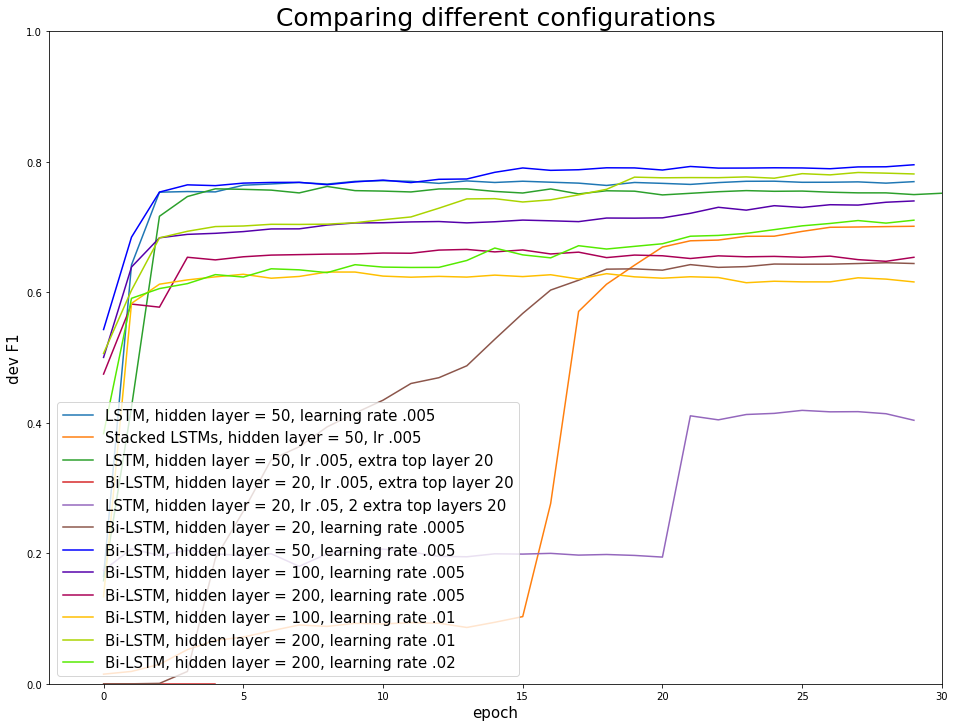
\includegraphics[width=330px]{figs/config_compar.png}
\caption{Comparing many different architectures and learning parameters led us to choose a \textbf{bi-LSTM} for the rest of our study. Some models with additional layers may have been able to perform as well with finer tuning, but we considered that the simpler would bring the most robustness}
\label{config_compar}
\end{center}
\end{figure}

\subsubsection{Dropout rate}

The first learning parameter we looked at in details is the dropout rate. It gives the portion of a layer's neurons we want arbitrarily desactivated at each pass over the network, and it's designed to give the network more robustness (because the neurons "learn" to not depend too much on each other). We find that the best performances, with everything else fixed, are achieved with a dropout rate around 20\%, as shown in Fig \ref{dr_devf1} --- comparing learning curves --- and Fig \ref{dr_graph} --- comparing best performances.

\begin{figure}[h!!]
\begin{center}
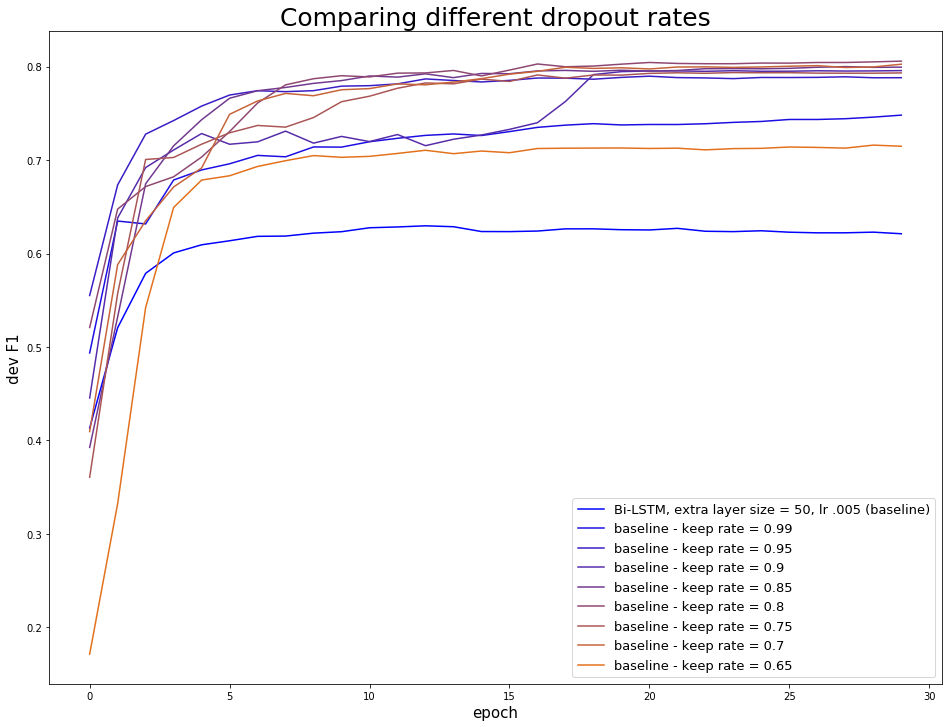
\includegraphics[width=350px]{figs/dr_devf1.png}
\caption{Learning curves for different dropout rates (dev set F1 score as a function of the number of epochs) ; we see that the most optimal dropout rate for learning is around 20\%}
\label{dr_devf1}
\end{center}
\end{figure}

\begin{figure}[h!]
\begin{center}
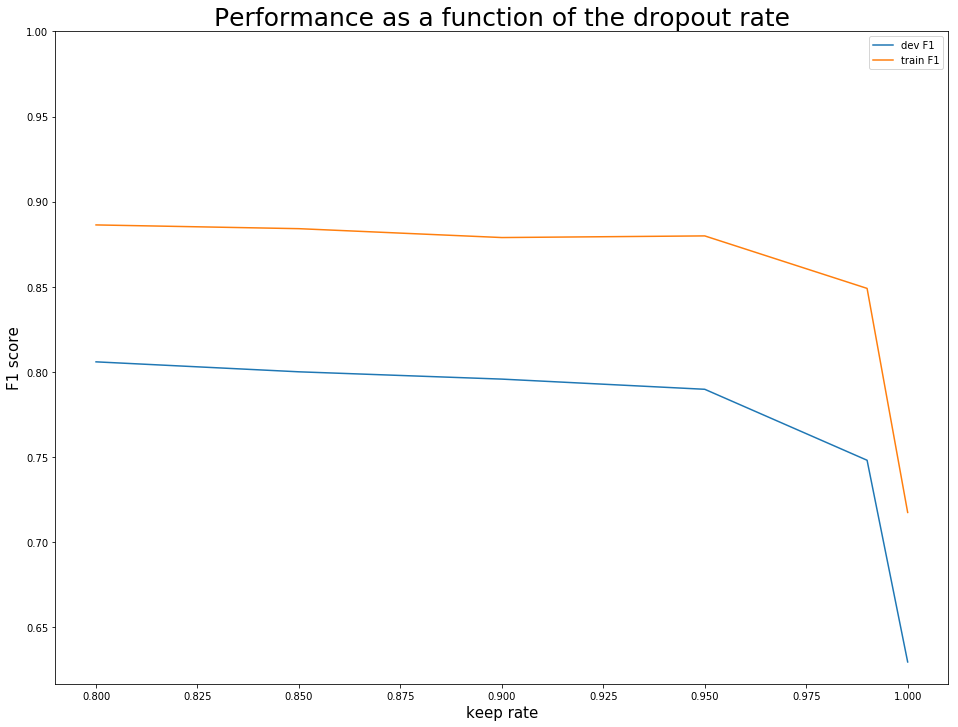
\includegraphics[width=250px]{figs/dr_graph.png}
\caption{Best performance of the model, as a function of the keep rate (1 - dropout rate)}
\label{dr_graph}
\end{center}
\end{figure}

\subsubsection{L2 regularization}

Once satisfied with our bi-LSTM model with 20\% dropout, we tried tuning L2 regularization, keeping everything else fixed.

L2 regularization can be written as follows: $$regularized~loss = loss + \beta~(||W_1||_2+||W_2||_2+...)$$ where the $W_j$ are the weights matrices involved in the model, and $\beta$ is the regularization hyper-parameter, which determines how strong we want to penalize large weights.

We tried a rather wide grid of values for $\beta$, and could compare each one's performance, both looking at the learning curves (Fig \ref{l2_devf1}) and at the best performance (Fig \ref{l2_graph}). Surprinsingly, the unregularized baseline is almost unbeatable. Still, we consider it sane to introduce some weight penalization, and therefore keep $\beta=3~10^{-5}$.


\begin{figure}[h!]
\begin{center}
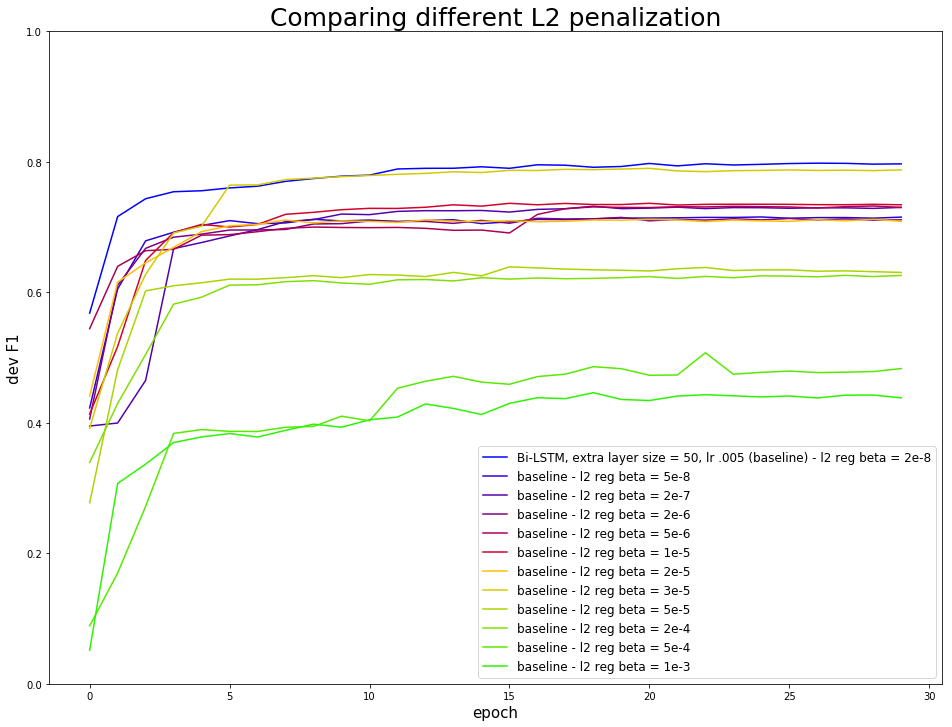
\includegraphics[width=350px]{figs/l2_devf1.png}
\caption{Learning curves for different $\beta$ values (dev set F1 score as a function of the number of epochs) ; we see that surprinsingly, few regularized models reach the out-of-sample performance of the unregularized baseline}
\label{l2_devf1}
\end{center}
\end{figure}

\begin{figure}[h!]
\begin{center}
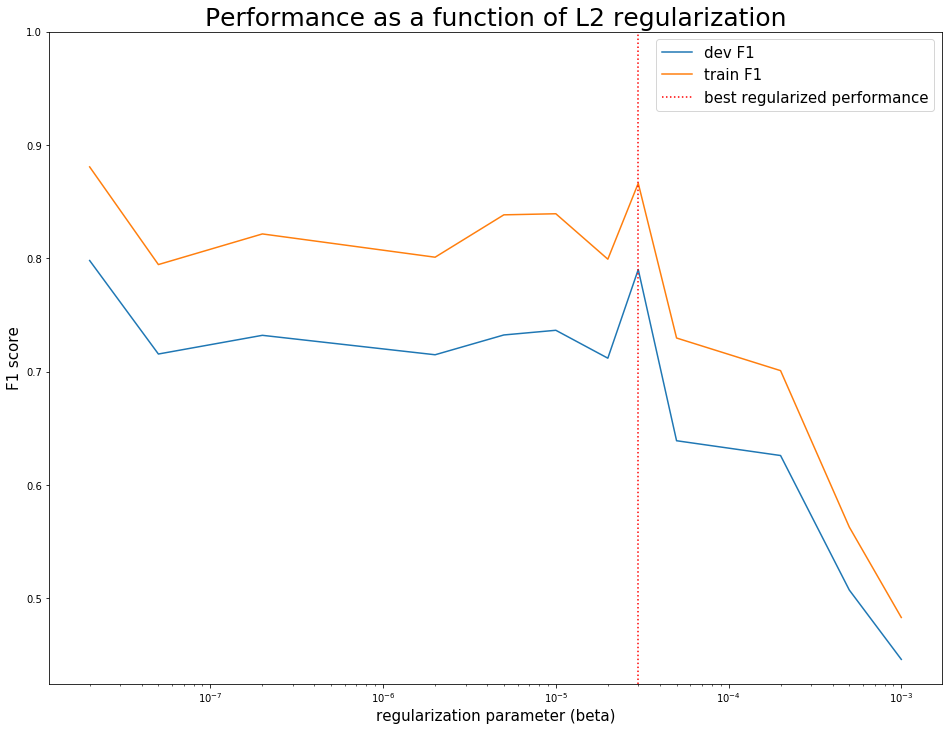
\includegraphics[width=250px]{figs/l2_graph.png}
\caption{Best performance of the model, as a function of the regularization parameter ; we select the most penalized model among the best performing ones.}
\label{l2_graph}
\end{center}
\end{figure}

\subsection{Incorporating the CRF}

We have tried to incorporate the prediction of a pre-trained CRF on top of two models: a simple LSTM model with $50$ recurrent cells, as well as our best-performing model, a Bidirectional LSTM. We have tried several values of the $\alpha$ parameter on an exponential scale, to see which one yields the best predicting performance. The $\alpha$ value which performs best on the train set is the one we will choose for evaluating our dev set.

We have summarized the results of varying the CRF's $\alpha$ parameter on a simple LSTM model in Fig \ref{lstm-crf-results}. First, we see that the dev $F_1$ performance curve closely follows the  train $F_1$ curve. This means that tuning the $\alpha$ parameter does not lead to an overfitting on specific subsets of the studied set. However, we obtain disappointing results on the contribution of the information of the CRF. The best results are obtained by not considering the CRF. Using more information from the CRF yields a steady decrease in $F_1$ performance.

It appears that the way we included the CRF in our model is not relevant for prediction. The information carried by the labels transition matrix $P$ is not predictive enough, and it is over-expressed compared to the Recurrent Network before being able to contribute in a constructive way.

\begin{figure}[h!]
\begin{center}
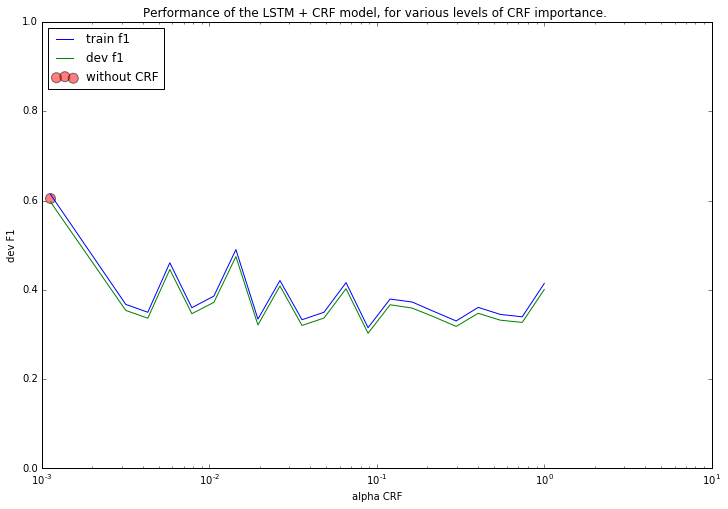
\includegraphics[width=250px]{figs/LSTM-CRF-vs-alpha.png}
\caption{Train and Dev set performance of a LSTM model, incorporating a CRF on the prediction step, versus the importance $\alpha$ given to the CRF. No positive level of importance yields superior performance. The best decision is not to use the extra information from the CRF. }
\label{lstm-crf-results}
\end{center}
\end{figure}

\section{Conclusion}

We have produced the following table to summarize our main results for each attempted technique.

\begin{center}
 \begin{tabular}{||c | c||}
 \hline
 Model  & Dev $F_1$ \\
 \hline\hline
 Naive word-by-word & $0.691$ \\
 \hline
 LSTM & $0.597$ \\
 \hline
 LSTM + CRF & $0.475$ \\
 \hline
 LSTM + extra layer & $0.770$ \\
 \hline
 LSTM + extra layer + CRF & $0.751$ \\
 \hline
 Bi-LSTM & $0.796$ \\ %[1ex]
 \hline
\end{tabular}
\end{center}

TODO

Opening :

- to enhance CRF, bidirectional CRF? Incorporating CRF on training?

- mention attention ?


\newpage
\bibliography{references}
\bibliographystyle{plain}

















%%\section{Submission of papers to NIPS 2013}
%%
%%NIPS requires electronic submissions.  The electronic submission site is
%%\begin{center}
%%   \url{http://papers.nips.cc}
%%\end{center}
%%
%%Please read carefully the
%%instructions below, and follow them faithfully.
%%\subsection{Style}
%%
%%Papers to be submitted to NIPS 2013 must be prepared according to the
%%instructions presented here. Papers may be only up to eight pages long,
%%including figures. Since 2009 an additional ninth page \textit{containing only
%%cited references} is allowed. Papers that exceed nine pages will not be
%%reviewed, or in any other way considered for presentation at the conference.
%%%This is a strict upper bound.
%%
%%Please note that this year we have introduced automatic line number generation
%%into the style file (for \LaTeXe and Word versions). This is to help reviewers
%%refer to specific lines of the paper when they make their comments. Please do
%%NOT refer to these line numbers in your paper as they will be removed from the
%%style file for the final version of accepted papers.
%%
%%The margins in 2013 are the same as since 2007, which allow for $\approx 15\%$
%%more words in the paper compared to earlier years. We are also again using
%%double-blind reviewing. Both of these require the use of new style files.
%%
%%Authors are required to use the NIPS \LaTeX{} style files obtainable at the
%%NIPS website as indicated below. Please make sure you use the current files and
%%not previous versions. Tweaking the style files may be grounds for rejection.
%%
%%%% \subsection{Double-blind reviewing}
%%
%%%% This year we are doing double-blind reviewing: the reviewers will not know
%%%% who the authors of the paper are. For submission, the NIPS style file will
%%%% automatically anonymize the author list at the beginning of the paper.
%%
%%%% Please write your paper in such a way to preserve anonymity. Refer to
%%%% previous work by the author(s) in the third person, rather than first
%%%% person. Do not provide Web links to supporting material at an identifiable
%%%% web site.
%%
%%%%\subsection{Electronic submission}
%%%%
%%%% \textbf{THE SUBMISSION DEADLINE IS MAY 31st, 2013. SUBMISSIONS MUST BE LOGGED BY
%%%% 23:00, MAY 31st, 2013, UNIVERSAL TIME}
%%
%%%% You must enter your submission in the electronic submission form available at
%%%% the NIPS website listed above. You will be asked to enter paper title, name of
%%%% all authors, keyword(s), and data about the contact
%%%% author (name, full address, telephone, fax, and email). You will need to
%%%% upload an electronic (postscript or pdf) version of your paper.
%%
%%%% You can upload more than one version of your paper, until the
%%%% submission deadline. We strongly recommended uploading your paper in
%%%% advance of the deadline, so you can avoid last-minute server congestion.
%%%%
%%%% Note that your submission is only valid if you get an e-mail
%%%% confirmation from the server. If you do not get such an e-mail, please
%%%% try uploading again.
%%
%%
%%\subsection{Retrieval of style files}
%%
%%The style files for NIPS and other conference information are available on the World Wide Web at
%%\begin{center}
%%   \url{http://www.nips.cc/}
%%\end{center}
%%The file \verb+nips2013.pdf+ contains these
%%instructions and illustrates the
%%various formatting requirements your NIPS paper must satisfy. \LaTeX{}
%%users can choose between two style files:
%%\verb+nips11submit_09.sty+ (to be used with \LaTeX{} version 2.09) and
%%\verb+nips11submit_e.sty+ (to be used with \LaTeX{}2e). The file
%%\verb+nips2013.tex+ may be used as a ``shell'' for writing your paper. All you
%%have to do is replace the author, title, abstract, and text of the paper with
%%your own. The file
%%\verb+nips2013.rtf+ is provided as a shell for MS Word users.
%%
%%The formatting instructions contained in these style files are summarized in
%%sections \ref{gen_inst}, \ref{headings}, and \ref{others} below.
%%
%%%% \subsection{Keywords for paper submission}
%%%% Your NIPS paper can be submitted with any of the following keywords (more than one keyword is possible for each paper):
%%
%%%% \begin{verbatim}
%%%% Bioinformatics
%%%% Biological Vision
%%%% Brain Imaging and Brain Computer Interfacing
%%%% Clustering
%%%% Cognitive Science
%%%% Control and Reinforcement Learning
%%%% Dimensionality Reduction and Manifolds
%%%% Feature Selection
%%%% Gaussian Processes
%%%% Graphical Models
%%%% Hardware Technologies
%%%% Kernels
%%%% Learning Theory
%%%% Machine Vision
%%%% Margins and Boosting
%%%% Neural Networks
%%%% Neuroscience
%%%% Other Algorithms and Architectures
%%%% Other Applications
%%%% Semi-supervised Learning
%%%% Speech and Signal Processing
%%%% Text and Language Applications
%%
%%%% \end{verbatim}
%%
%%\section{General formatting instructions}
%%\label{gen_inst}
%%
%%The text must be confined within a rectangle 5.5~inches (33~picas) wide and
%%9~inches (54~picas) long. The left margin is 1.5~inch (9~picas).
%%Use 10~point type with a vertical spacing of 11~points. Times New Roman is the
%%preferred typeface throughout. Paragraphs are separated by 1/2~line space,
%%with no indentation.
%%
%%Paper title is 17~point, initial caps/lower case, bold, centered between
%%2~horizontal rules. Top rule is 4~points thick and bottom rule is 1~point
%%thick. Allow 1/4~inch space above and below title to rules. All pages should
%%start at 1~inch (6~picas) from the top of the page.
%%
%%%The version of the paper submitted for review should have ``Anonymous Author(s)'' as the author of the paper.
%%
%%For the final version, authors' names are
%%set in boldface, and each name is centered above the corresponding
%%address. The lead author's name is to be listed first (left-most), and
%%the co-authors' names (if different address) are set to follow. If
%%there is only one co-author, list both author and co-author side by side.
%%
%%Please pay special attention to the instructions in section \ref{others}
%%regarding figures, tables, acknowledgments, and references.
%%
%%\section{Headings: first level}
%%\label{headings}
%%
%%First level headings are lower case (except for first word and proper nouns),
%%flush left, bold and in point size 12. One line space before the first level
%%heading and 1/2~line space after the first level heading.
%%
%%\subsection{Headings: second level}
%%
%%Second level headings are lower case (except for first word and proper nouns),
%%flush left, bold and in point size 10. One line space before the second level
%%heading and 1/2~line space after the second level heading.
%%
%%\subsubsection{Headings: third level}
%%
%%Third level headings are lower case (except for first word and proper nouns),
%%flush left, bold and in point size 10. One line space before the third level
%%heading and 1/2~line space after the third level heading.
%%
%%\section{Citations, figures, tables, references}
%%\label{others}
%%
%%These instructions apply to everyone, regardless of the formatter being used.
%%
%%\subsection{Citations within the text}
%%
%%Citations within the text should be numbered consecutively. The corresponding
%%number is to appear enclosed in square brackets, such as [1] or [2]-[5]. The
%%corresponding references are to be listed in the same order at the end of the
%%paper, in the \textbf{References} section. (Note: the standard
%%\textsc{Bib\TeX} style \texttt{unsrt} produces this.) As to the format of the
%%references themselves, any style is acceptable as long as it is used
%%consistently.
%%
%%As submission is double blind, refer to your own published work in the
%%third person. That is, use ``In the previous work of Jones et al.\ [4]'',
%%not ``In our previous work [4]''. If you cite your other papers that
%%are not widely available (e.g.\ a journal paper under review), use
%%anonymous author names in the citation, e.g.\ an author of the
%%form ``A.\ Anonymous''.
%%
%%
%%\subsection{Footnotes}
%%
%%Indicate footnotes with a number\footnote{Sample of the first footnote} in the
%%text. Place the footnotes at the bottom of the page on which they appear.
%%Precede the footnote with a horizontal rule of 2~inches
%%(12~picas).\footnote{Sample of the second footnote}
%%
%%\subsection{Figures}
%%
%%All artwork must be neat, clean, and legible. Lines should be dark
%%enough for purposes of reproduction; art work should not be
%%hand-drawn. The figure number and caption always appear after the
%%figure. Place one line space before the figure caption, and one line
%%space after the figure. The figure caption is lower case (except for
%%first word and proper nouns); figures are numbered consecutively.
%%
%%Make sure the figure caption does not get separated from the figure.
%%Leave sufficient space to avoid splitting the figure and figure caption.
%%
%%You may use color figures.
%%However, it is best for the
%%figure captions and the paper body to make sense if the paper is printed
%%either in black/white or in color.
%%\begin{figure}[h]
%%\begin{center}
%%%\framebox[4.0in]{$\;$}
%%\fbox{\rule[-.5cm]{0cm}{4cm} \rule[-.5cm]{4cm}{0cm}}
%%\end{center}
%%\caption{Sample figure caption.}
%%\end{figure}
%%
%%\subsection{Tables}
%%
%%All tables must be centered, neat, clean and legible. Do not use hand-drawn
%%tables. The table number and title always appear before the table. See
%%Table~\ref{sample-table}.
%%
%%Place one line space before the table title, one line space after the table
%%title, and one line space after the table. The table title must be lower case
%%(except for first word and proper nouns); tables are numbered consecutively.
%%
%%\begin{table}[t]
%%\caption{Sample table title}
%%\label{sample-table}
%%\begin{center}
%%\begin{tabular}{ll}
%%\multicolumn{1}{c}{\bf PART}  &\multicolumn{1}{c}{\bf DESCRIPTION}
%%\\ \hline \\
%%Dendrite         &Input terminal \\
%%Axon             &Output terminal \\
%%Soma             &Cell body (contains cell nucleus) \\
%%\end{tabular}
%%\end{center}
%%\end{table}
%%
%%\section{Final instructions}
%%Do not change any aspects of the formatting parameters in the style files.
%%In particular, do not modify the width or length of the rectangle the text
%%should fit into, and do not change font sizes (except perhaps in the
%%\textbf{References} section; see below). Please note that pages should be
%%numbered.
%%
%%\section{Preparing PostScript or PDF files}
%%
%%Please prepare PostScript or PDF files with paper size ``US Letter'', and
%%not, for example, ``A4''. The -t
%%letter option on dvips will produce US Letter files.
%%
%%Fonts were the main cause of problems in the past years. Your PDF file must
%%only contain Type 1 or Embedded TrueType fonts. Here are a few instructions
%%to achieve this.
%%
%%\begin{itemize}
%%
%%\item You can check which fonts a PDF files uses.  In Acrobat Reader,
%%select the menu Files$>$Document Properties$>$Fonts and select Show All Fonts. You can
%%also use the program \verb+pdffonts+ which comes with \verb+xpdf+ and is
%%available out-of-the-box on most Linux machines.
%%
%%\item The IEEE has recommendations for generating PDF files whose fonts
%%are also acceptable for NIPS. Please see
%%\url{http://www.emfield.org/icuwb2010/downloads/IEEE-PDF-SpecV32.pdf}
%%
%%\item LaTeX users:
%%
%%\begin{itemize}
%%
%%\item Consider directly generating PDF files using \verb+pdflatex+
%%(especially if you are a MiKTeX user).
%%PDF figures must be substituted for EPS figures, however.
%%
%%\item Otherwise, please generate your PostScript and PDF files with the following commands:
%%\begin{verbatim}
%%dvips mypaper.dvi -t letter -Ppdf -G0 -o mypaper.ps
%%ps2pdf mypaper.ps mypaper.pdf
%%\end{verbatim}
%%
%%Check that the PDF files only contains Type 1 fonts.
%%%For the final version, please send us both the Postscript file and
%%%the PDF file.
%%
%%\item xfig "patterned" shapes are implemented with
%%bitmap fonts.  Use "solid" shapes instead.
%%\item The \verb+\bbold+ package almost always uses bitmap
%%fonts.  You can try the equivalent AMS Fonts with command
%%\begin{verbatim}
%%\usepackage[psamsfonts]{amssymb}
%%\end{verbatim}
%% or use the following workaround for reals, natural and complex:
%%\begin{verbatim}
%%\newcommand{\RR}{I\!\!R} %real numbers
%%\newcommand{\Nat}{I\!\!N} %natural numbers
%%\newcommand{\CC}{I\!\!\!\!C} %complex numbers
%%\end{verbatim}
%%
%%\item Sometimes the problematic fonts are used in figures
%%included in LaTeX files. The ghostscript program \verb+eps2eps+ is the simplest
%%way to clean such figures. For black and white figures, slightly better
%%results can be achieved with program \verb+potrace+.
%%\end{itemize}
%%\item MSWord and Windows users (via PDF file):
%%\begin{itemize}
%%\item Install the Microsoft Save as PDF Office 2007 Add-in from
%%\url{http://www.microsoft.com/downloads/details.aspx?displaylang=en\&familyid=4d951911-3e7e-4ae6-b059-a2e79ed87041}
%%\item Select ``Save or Publish to PDF'' from the Office or File menu
%%\end{itemize}
%%\item MSWord and Mac OS X users (via PDF file):
%%\begin{itemize}
%%\item From the print menu, click the PDF drop-down box, and select ``Save
%%as PDF...''
%%\end{itemize}
%%\item MSWord and Windows users (via PS file):
%%\begin{itemize}
%%\item To create a new printer
%%on your computer, install the AdobePS printer driver and the Adobe Distiller PPD file from
%%\url{http://www.adobe.com/support/downloads/detail.jsp?ftpID=204} {\it Note:} You must reboot your PC after installing the
%%AdobePS driver for it to take effect.
%%\item To produce the ps file, select ``Print'' from the MS app, choose
%%the installed AdobePS printer, click on ``Properties'', click on ``Advanced.''
%%\item Set ``TrueType Font'' to be ``Download as Softfont''
%%\item Open the ``PostScript Options'' folder
%%\item Select ``PostScript Output Option'' to be ``Optimize for Portability''
%%\item Select ``TrueType Font Download Option'' to be ``Outline''
%%\item Select ``Send PostScript Error Handler'' to be ``No''
%%\item Click ``OK'' three times, print your file.
%%\item Now, use Adobe Acrobat Distiller or ps2pdf to create a PDF file from
%%the PS file. In Acrobat, check the option ``Embed all fonts'' if
%%applicable.
%%\end{itemize}
%%
%%\end{itemize}
%%If your file contains Type 3 fonts or non embedded TrueType fonts, we will
%%ask you to fix it.
%%
%%\subsection{Margins in LaTeX}
%%
%%Most of the margin problems come from figures positioned by hand using
%%\verb+\special+ or other commands. We suggest using the command
%%\verb+\includegraphics+
%%from the graphicx package. Always specify the figure width as a multiple of
%%the line width as in the example below using .eps graphics
%%\begin{verbatim}
%%   \usepackage[dvips]{graphicx} ...
%%   \includegraphics[width=0.8\linewidth]{myfile.eps}
%%\end{verbatim}
%%or % Apr 2009 addition
%%\begin{verbatim}
%%   \usepackage[pdftex]{graphicx} ...
%%   \includegraphics[width=0.8\linewidth]{myfile.pdf}
%%\end{verbatim}
%%for .pdf graphics.
%%See section 4.4 in the graphics bundle documentation (\url{http://www.ctan.org/tex-archive/macros/latex/required/graphics/grfguide.ps})
%%
%%A number of width problems arise when LaTeX cannot properly hyphenate a
%%line. Please give LaTeX hyphenation hints using the \verb+\-+ command.
%%
%%
%%\subsubsection*{Acknowledgments}
%%
%%Use unnumbered third level headings for the acknowledgments. All
%%acknowledgments go at the end of the paper. Do not include
%%acknowledgments in the anonymized submission, only in the
%%final paper.
%%
%%\subsubsection*{References}
%%
%%References follow the acknowledgments. Use unnumbered third level heading for
%%the references. Any choice of citation style is acceptable as long as you are
%%consistent. It is permissible to reduce the font size to `small' (9-point)
%%when listing the references. {\bf Remember that this year you can use
%%a ninth page as long as it contains \emph{only} cited references.}
%%
%%\small{
%%[1] Alexander, J.A. \& Mozer, M.C. (1995) Template-based algorithms
%%for connectionist rule extraction. In G. Tesauro, D. S. Touretzky
%%and T.K. Leen (eds.), {\it Advances in Neural Information Processing
%%Systems 7}, pp. 609-616. Cambridge, MA: MIT Press.
%%
%%[2] Bower, J.M. \& Beeman, D. (1995) {\it The Book of GENESIS: Exploring
%%Realistic Neural Models with the GEneral NEural SImulation System.}
%%New York: TELOS/Springer-Verlag.
%%
%%[3] Hasselmo, M.E., Schnell, E. \& Barkai, E. (1995) Dynamics of learning
%%and recall at excitatory recurrent synapses and cholinergic modulation
%%in rat hippocampal region CA3. {\it Journal of Neuroscience}
%%{\bf 15}(7):5249-5262.
%%}

\end{document}
